\section{Theory}
\label{chap:Theory}

\subsection{Gradient Decedent}
\label{chap:Gradient Decedent}

\quad \, Gradient descent (GD) or Batch gradient descent (BGD) is a first-order method for finding a local or global minimum of a multi-variable differentiable function. To do that, it takes negative gradient steps of a function at a current point. We denote here ($\boldsymbol{w_{0}}$) as the initial/start point, and the processes are described as $w_{n+1} &= w_{n} - \eta \nabla_{\boldsymbol{w}} f(\boldsymbol{w_{n}})$, where $\eta \in \mathbb{R}$ is the Learning Rate which must be small enough; $\nabla f(w_{n})$ is the gradient of the cost function (MSE); $\boldsymbol{w}$ is the set of coefficients or weights.\\

It is important to remark that the Leaning rate ($\eta$) is the step size or amount of the gradient that will update the weights of the model during training. Brilliant illustrations were extracted from \hyperref[Bib:Hands-on Machine Learning]{[3]}[p. 157] to visually explain the effect of a too-small Learning rate or too large learning rate:

\begin{figure}[H]
\label{fig:fig1}
\centering
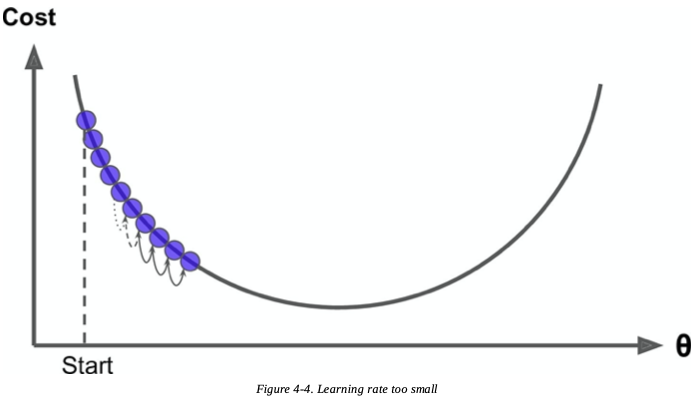
\includegraphics[width=7cm]{eta_too_small}
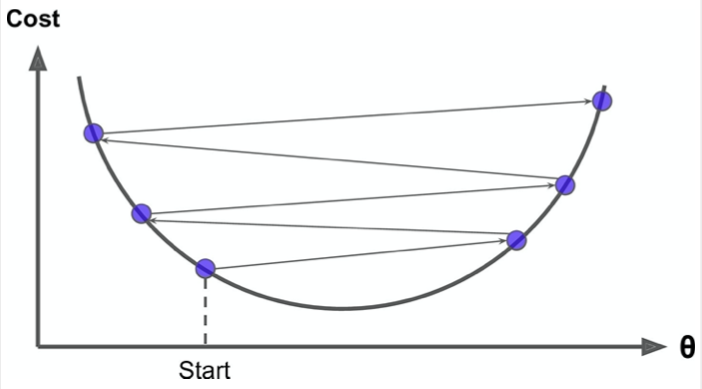
\includegraphics[width=7cm]{eta_too_large}
\caption{Left-illustration visually demonstrates the effect of a too-small learning rate. Right-illustration visually demonstrates the effect of a too-large learning rate.}
\end{figure}

In summary, the algorithm will need many iterations to achieve the local or global minimum if the learning rate is too low. On the other hand, if the learning rate is too large, the algorithm diverges and never achieves the local or global minimum.\\

The MSE cost-function is utilized to compute the linear regression case gradient, which also is excellent for these cases because it is a convex continuous function. This continuity and convexity properties mean that the gradient descent will always go in the local or global minimum direction as illustrated under:

\begin{figure}[H]
\label{fig:fig2}
\centering
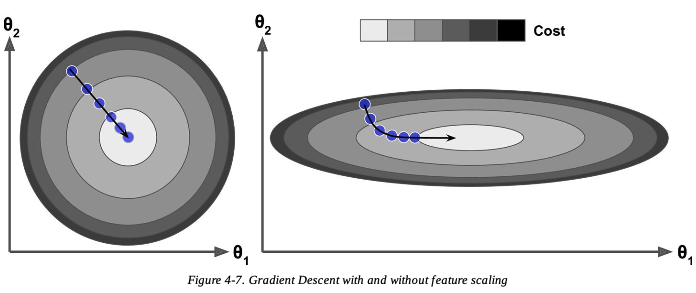
\includegraphics[height=5cm]{mse_cost_gradient}
\caption{Figures extracted from \hyperref[Bib:Hands-on Machine Learning]{[3]}[p. 159]. Left-side figure shows a fast Gradient Descent on a training set where features 1 and 2 have the same scale. Right-side figure shows a slower Gradient Descent on a training set where feature 1 has smaller values than feature 2.}
\end{figure}

From Calculus, the gradient of MSE can be calculated as:\\

\begin{align*}
w_{n+1} &= w_{n} - \eta \nabla_{\boldsymbol{w}} f(\boldsymbol{w_{n}})\\
&= w_{n} - \eta * (\frac{2}{m}*\boldsymbol{X}.T*(\boldsymbol{X}*\boldsymbol{w}-\boldsymbol{z}))
\end{align*}

\noindent where $\boldsymbol{X}$ is the design matrix with explanatory variables; $\boldsymbol{z}$ is the set with response variables; $n=[0, 1, 2, ..., m], n \in \mathbb{N}$ is the number of steps/interactions/epochs.\\

The algorithm called \href{https://github.com/fabiorodp/UiO-FYS-STK4155/blob/master/Project2/package/gradient_descent.py}{BGDM} in \href{https://github.com/fabiorodp/UiO-FYS-STK4155/blob/master/Project2/package/}{package/} directory, when the parameter gamma=0, performs this method, which initializes its' initial points or weights randomly. Then, the gradient is calculated for every epoch and decreased from those weights described above. It is essential to state that the \href{https://github.com/fabiorodp/UiO-FYS-STK4155/blob/master/Project2/package/gradient_descent.py}{BGDM} computes an entire batch's gradient, which means a unique block containing all training data samples and features (design matrix $\boldsymbol{X}$).

\subsubsection{Learning Rate ($\eta$) with decay/schedule}
\label{chap:Learning Rate with decay}

\quad \, The Learning Rate ($\eta$) with decay/schedule changes during learning between epochs/interactions. There are many different types of $\eta$ schedules; however, we will focus on the most used one called time-based. For that, a parameter decay is introduced, and it will alter $\eta$ depending on the learning rate of the previous time iteration according to the mathematical formula:

\begin{align*}
\eta_{n+1} = \frac{\eta_n}{1 + decay * epoch}
\end{align*}

\noindent where $\eta_{n+1}$ is the learning rate with decay; $\eta_n$ is the previous learning rate; decay is a constant parameter; epoch is the step index.

\subsubsection{Stochastic Gradient Decedent}
\label{chap:Stochastic Gradient Decedent}

\quad \, Stochastic Gradient Decedent (SGD) is a stochastic approximation of the gradient descent. It replaces the gradient from (BGD), calculated from an entire data set $\boldsymbol{X}$, by a gradient calculated from a randomly selected feature vector of a sample from the data set $\boldsymbol{X}$. Put differently, the main difference between BGD and SGD is that the former updates its weights after the entire data-set gradient computation. The latter updates its weights after every unique sample and its features.

\begin{figure}[H]
\label{fig:fig3}
\centering
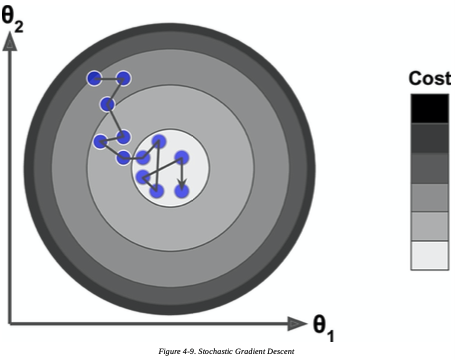
\includegraphics[height=5cm]{sgd_gradient}
\caption{Figure extracted from \hyperref[Bib:Hands-on Machine Learning]{[3]}[p. 163] illustrating the effect of the SGD during training.}
\end{figure}

Therefore, SGD is faster than BGD. However, as \hyperref[fig:fig3]{Fig.3} shows, due to SGD's stochastic nature, the gradient is much less regular, as stated by \textit{Aurélien Géron} in \hyperref[Bib:Hands-on Machine Learning]{[3]}[p. 163] "\textit{instead of gently decreasing until reaches the minimum, the cost function will bounce up and down, decreasing only on average. Over time it will end up very close to the minimum, but once it gets there it will continue to bounce around, never settling down. So once the algorithm stops, the final parameter values are good, but not optimal}".\\

The algorithm called \href{https://github.com/fabiorodp/UiO-FYS-STK4155/blob/master/Project2/package/gradient_descent.py}{MiniSGDM} in \href{https://github.com/fabiorodp/UiO-FYS-STK4155/blob/master/Project2/package/}{package/} directory, when parameters gamma=0 and batch-size=1, performs the method above.

\subsubsection{Mini-batch Stochastic Gradient Decedent}
\label{chap:Mini-batch Stochastic Gradient Decedent}

\quad \, Mini-batch Stochastic Gradient Decedent (Mini-SGD) differs from SGD in the number of samples and its features picked randomly. The former uses blocks of mini-batches containing more than 1 sample and its features from the data-set x, then the number of blocks of mini-batches will be the total of samples divided by the fixed size of the mini-batches. This process reduces the number of times the weights update turning the system faster than BGD and SGD. Therefore, Mini-batch SGD has tremendous benefits over BGD and SGD, especially in high-dimensional optimization problems, because it reduces the time and computation's cost resulting in a faster fitting for the model without losing the accuracy.\\

The algorithm called \href{https://github.com/fabiorodp/UiO-FYS-STK4155/blob/master/Project2/package/gradient_descent.py}{MiniSGDM} in \href{https://github.com/fabiorodp/UiO-FYS-STK4155/blob/master/Project2/package/}{package/} directory, when parameters gamma=0 and batch-size $> 1$, performs the method above.

\subsubsection{BGD, SGD and Mini-batch SGD with momentum}
\label{chap:BGD, SGD and Mini-batch SGD with momentum}

\quad \, BGD, SGD and Mini-batch SGD can be used with a momentum parameter ($0 < \gamma <= 1$) that plays the role of a memory of the gradient steps' direction \hyperref[Bib:Week40Notes]{[4]}, as follows:

\begin{align*}
\boldsymbol{v}_{n+1} = \gamma \boldsymbol{v}_{n} + \eta_{n+1} \nabla_{\boldsymbol{w}} f(\boldsymbol{w_{n}})
\end{align*}

\noindent where $\boldsymbol{w}_{n+1} = \boldsymbol{w}_{n} - \boldsymbol{v}_{n}$; $\boldsymbol{v}_{n}$ is a running average of recently encountered weights \hyperref[Bib:Week40Notes]{[4]}.\\

The algorithms called \href{https://github.com/fabiorodp/UiO-FYS-STK4155/blob/master/Project2/package/gradient_descent.py}{BGDM and MiniSGDM} in \href{https://github.com/fabiorodp/UiO-FYS-STK4155/blob/master/Project2/package/}{package/} directory, when parameter $0 < \gamma <= 1$, perform the method above.


\subsection{Deep Neural Networks}
\label{chap:Deep Neural Networks}

\quad \, The deep neural network (DNN) is part of the neural network (NN) and machine learning (ML). \textit{Sebastian Raschka} and \textit{Vahid Mirjalili} define deep learning in \hyperref[Bib:Python Machine Learning]{[2]}[p. 542] as "\textit{understood as a set of algorithms that were developed to train artificial neural networks with many layer most efficiently}".\\

Before start our study of DNN we need to understand the process for a simple NN. In \hyperref[Bib:Python Machine Learning]{[2]}[p. 547] has a brilliant picture illustrating the Adaptive Linear Neuron (Adaline algorithm) which resembles in part the processes of a NN:

\begin{figure}[H]
\label{fig:fig4}
\centering
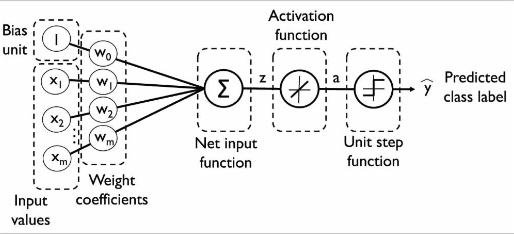
\includegraphics[height=5cm]{nn_process}
\caption{Figure extracted from \hyperref[Bib:Python Machine Learning]{[2]}[p. 547] illustrating Adaline process.}
\end{figure}

Our project's scope is not to explain the Adaline process, but, in a straightforward explanation, the process consists in, for every epoch, a matrix multiplication between training data and weights plus bias, which the result is called net input. Then it is submitted to an activation function to compute the gradient update and update the weights for the next epoch or obtain the prediction. For more details about Adaline, see \hyperref[Bib:Python Machine Learning]{[2]}[Chapter 2].\\

This process is very similar to the NN, but only considers an input layer connected to the output layer without any hidden layer. The difference between this process and the NN process is that NN has a hidden-layer between the input and output layers. In other words, Adaline has two layers, and NN has three layers in total. Regarding DNN, it has an input layer, two or more hidden layers, and output layer. The illustration for NN follows:

\begin{figure}[H]
\label{fig:fig5}
\centering
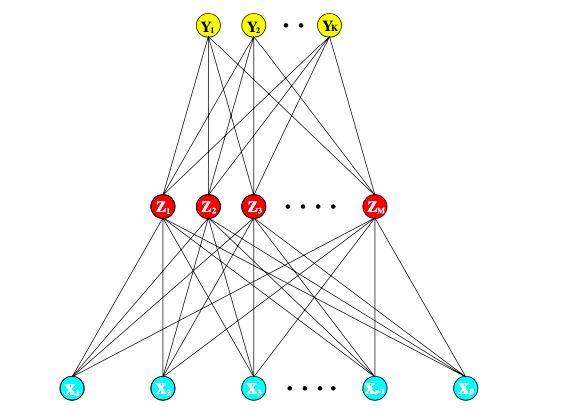
\includegraphics[height=5cm]{single_hidden_layer}
\caption{Figure extracted from \hyperref[Bib:The Elements Of Statistical Learning DataMining]{[1]}[p. 393] illustrating the connections of a Neural Network. The circles represent nodes/neurons. Green-circles, red-circles, and  Yellow-circles are the neurons for the input, hidden, and output layers, respectively.}
\end{figure}

The way that NN connects the input-layer to the hidden-layer and output-layer is called Feed-forward. The method to update the weights is called back-propagation.

\subsubsection{Feed-Forward}
\label{chap:Feed-Forward}

\quad \, The computations of the connections between input, hidden, and output layers are made by a technique called feed-forward (FFNN), illustrated in \hyperref[fig:fig5]{Fig.5}. Basically, for each training instance (mini-batch containing vectors of features denoted by $\textbf{x}$), the algorithm computes the net input ($\textbf{z}$) throughout matrix-vector multiplications between inputs ($\textbf{a}^{[input]}$) and weights ($\textbf{w}$) plus bias ($\textbf{b}$). The net input ($\textbf{z}$) will be submitted to an activation function, and its results/output are denoted by ($\textbf{a}^{[output]}$), such that:

\begin{align*}
\textbf{x} = \textbf{a}^{[input]} \rightarrow \sum_{j=1}^{M} \textbf{w}_{ij} \textbf{a}^{[input]} + \textbf{b}_i = \textbf{z}
\rightarrow f(\textbf{z}) = \textbf{a}^{[output]}
\end{align*}

\noindent where $i :=$ each node in the single hidden-layer; $j :=$ each node in the input/output layer.\\

Now, suppose we have a DNN with multiple hidden-layers. Hence, the FFDNN mathematical generalization will be:

\begin{align*}
\textbf{x} = \textbf{a}^{[0]} \rightarrow f^{l+1}\left[\!\sum_{j=1}^{N_l} w_{ij}^3 f^l\left(\sum_{k=1}^{N_{l-1}}w_{jk}^{l-1}\left(\dots f^1\left(\sum_{n=1}^{N_0} w_{mn}^1 \textbf{a}^{[0]}+ b_m^1\right)\dots\right)+b_k^2\right)+b_1^3\right] = a^{l+1}_i
\end{align*}

\noindent which illustrates FFDNN property \hyperref[Bib:Week40Notes]{[4]} of a Multi-layer perceptrons (MLP).\\

\subsubsection{Back-propagation}
\label{chap:Back-propagation}

\quad \, After the FF process, the output layer contains the predictions of the model. Next, the model compares the predictions and the real targets by applying a specific loss-function. Based on the loss-function results, the system will update the weights and bias, improving the performance by mini-batch stochastic gradient descent. Typically, the model initializes the weights and bias randomly, resulting in bad predictions initially. Still, as soon as the weights and bias are updated, the loss decreases to a local or global minimum, and the predictions get more accurate.\\

As said, back-propagation is the method of how the model will update the weights and bias. Now, the computations occur from the output layer to the input layer in a backward process. Utilizing the chosen loss-function (C) and by the chain rule \hyperref[Bib:Hands-on Machine Learning]{[3]}[p.396], the output error $\delta_L$ is:

\begin{align*}
\delta^{[l]} = \frac{\partial C}{\partial a^{[l]}} * \frac{\partial a^{[l]}}{\partial z^{[l]}},
\end{align*}

\noindent and the error for the other hidden-layers is:\\

\begin{align*}
\delta^{[l]} = \delta^{[l-1]} W^{[l-1].T} [f(z^{[l]})]_W^',
\end{align*}

\noindent where $f^'$ is the derivative of the activation function utilized.\\

Hence, the update of the weights and biases are:

$$W^{[l-1]} = W^{[l-1]} - \eta a^{[l-1].T} \delta^{[l]}$$
$$b^{[l-1]} = b^{[l-1]} - \eta \delta^{[l]},$$

\noindent where $\eta$ is the learning step.\\

After every epoch, the processes FF and back-propagation are performed forwards predicting the target and backward updating the weights and bias. The mini-batch trick is also applied to reduce the cost of the computations.

\subsubsection{The vanishing or exploding gradient problems}
\label{chap:The vanishing or exploding gradient problems}

\quad \, As discussed before, the back-propagation algorithm goes from the output layer to the input layer, calculating the cost gradient and updating weights and biases by the gradient descent steps.\\

Unfortunately, these gradients may vanish or explode \hyperref[Bib:Hands-on Machine Learning]{[3]}[p. 369] somehow. Typically, it gets smaller and smaller as its progress throughout lower layers, resulting in not updating the weights and biases and never converging to a good solution. Conversely, the gradient can also grow bigger and bigger, diverging the weights and biases updates. These are investigated as the vanishing and exploding gradient problems \hyperref[Bib:Hands-on Machine Learning]{[3]}[p. 369], respectively.\\

The researchers tackle these problems by applying different activation functions for hidden-layers (Sigmoid, Tanh, ReLu, etc.) or initializing the weights and biases with several methods (Gaussian distribution, Xavier method, etc.). We will cover these topics in the next sub-sections.

\subsubsection{Sigmoid}
\label{chap:Sigmoid}

\quad \, Sigmoid is a mathematical function with a shape of an "S"-curve widely used in logistic regression, NN and DNN because returns values between 0 and 1, such that:

\begin{align*}
f(z) = \frac{1}{1 + e^{-z}} = \frac{e^{z}}{e^{z}+1}
\end{align*}

The derivative of the Sigmoid is:

\begin{align*}
f^{'}(z) = f(z) (1 - f(z))
\end{align*}

This function replaced the originally step function of the MLP, because the latter contains only flat segments in which the gradient technique does not work \hyperref[Bib:Hands-on Machine Learning]{[3]}[p.351]. The former, Sigmoid, has a well-defined nonzero derivative everywhere, allowing the Gradient descent to work correctly in every step. Still, it may have problems because of its saturation when results are near zero, vanishing the gradient descent step. Therefore, another technique was introduced, hyperbolic Tanh, trying to avoid that.

\subsubsection{Hyperbolic tanh}
\label{chap:Hyperbolic tanh}

\quad \, Like the Sigmoid, the hyperbolic tangent function tanh is S-shaped, continuous, and differentiable. This method was implemented to avoid vanishing the gradient descent step due to its range between [-1, 1]. Besides, the hyperbolic Tanh helps to speed up convergence because of its centered values on 0 \hyperref[Bib:Hands-on Machine Learning]{[3]}[p. 351].\\

The mathematical representation:

\begin{align*}
f(z) = \frac{e^{z} - e^{-z}}{e^{z} + e^{-z}}
\end{align*}

Its derivative:

\begin{align*}
f^{'}(z) = 1 - f(z)^2
\end{align*}

\subsubsection{Rectified Linear Unit (ReLu)}
\label{chap:Rectified Linear Unit}

\quad \, ReLu is a continuous and differentiable function, except when z=0, when the slope changes abruptly, and the gradient descent bounce around \hyperref[Bib:Hands-on Machine Learning]{[3]}[p. 351]. Nevertheless, the function works excellently as an activation function and has faster computations than Sigmoid or Tanh. Besides, it does not have a maximum output value helping overcoming problems with the Gradient descent.\\

The mathematical representation:

\begin{align*}
f(z) = 
\begin{cases}
0,  &  z < 0\\
z,  & \text{otherwise}
\end{cases}
\end{align*}

\subsubsection{Softmax}
\label{chap:Softmax}

\quad \, Softmax function returns the estimated probability of the corresponding prediction class. It is a generalized approach to support multiple class predictions without training and combining various binary classifiers.\\

The mathematical representation:

\begin{align*}
\sigma(z)_i = \frac{e^z_i}{\sum_{j=1}^{K} e^{z_j}},
\end{align*}

\noindent for $i=1, ..., K$ and $z=(z_1, ..., z_K) \in R^K$.

\subsubsection{Xavier and He weights initialization method}
\label{chap:Xavier and He weights initialization method}

\quad \, According to \hyperref[Bib:XavierHe]{[6]} paper, the authors verified and discussed the variance of the output layer on Neural Networks. They noticed that the output layer typically has a higher variance than the input layer has, and it might be a problem.\\

Thus, for the Feed-forward and back-propagation processes flow correctly, it is necessary the same variance for the input, output layers as well as for the gradients \hyperref[Bib:Hands-on Machine Learning]{[3]}[p. 371].\\

For that, it was proposed to initialize the parameters of the model using a specific strategy of each type of activation function, as follows:

\begin{figure}[H]
\label{fig:xavier}
\centering
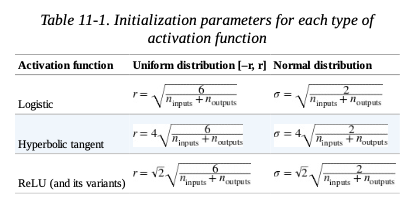
\includegraphics[height=5cm]{xavier_init}
\caption{Types of Xavier initialization. Picture extracted from \hyperref[Bib:Hands-on Machine Learning]{[3]}[p. 371]}
\end{figure}


\subsection{Logistic Regression}
\label{chap:Logistic Regression}

\quad \, Logistic regression models the probability that input data ($\textbf{x}$) leads to outcomes ($y_i$), for $i=1, 2, ..., m$, where $m$ is the number of possible labels for the outcome classes and $y_i \in [0, 1]$. By using the Sigmoid function, it expresses these probabilities of two outcomes labels, i.e. 0 and 1, as follows:

$$p(y_i=1|x_i, \beta) = \frac{e^{\beta^T x_i}}{1+e^{\beta^T x_i}}$$
$$p(y_i=0|x_i, \beta) = 1 - p(y_i = 1|x_i, \beta),$$

\noindent where $\beta$ are the coefficients that will be estimated by the model.\\

We define $D=(x_i, y_i)$ and assume that the samples are independent identically distributed (i.i.d.). The total likelihood for all possible outcomes in $D$ is approximated by the product of its individual probabilities for a particular outcome $y_i$:

\begin{align*}
P(D|\beta) = \prod_{i=1}^{n} \left[ p(y_i= 1 | x_i, \beta \right]^{y_i} \left[ 1 - p(y_i= 1 | x_i, \beta) \right]^{1 - y_i}
\end{align*}

From the Maximum Likelihood Estimation principle, the log of the above equation is taken, leading to the log-likelihood below:

\begin{align*}
\log P(D|\beta) = \sum_{i=1}^n \left[ y_i \log p(y_i = 1| x_i, \beta) + (1 - y_i)\log(1 - p(y_i = 1 | x_i, \beta))\right]
\end{align*}

By reordering the expression above and multiplying by -1, we end up with the cross-entropy expression:

\begin{align*}
C(\beta) = - \sum_{i=1}^n \left[ y_i\beta^Tx_i - \log(1 + \exp(\beta^Tx_i)) \right],
\end{align*}

\noindent which is the cost-function for the logistic regression.\\

Next, it is minimized the cross-entropy which is the same as maximizing the log-likelihood:

\begin{align*}
\frac{\partial C(\beta)}{\partial \beta} = - \sum_{i=1}^n x_i(y_i - p(y_i=1 | x_i, \beta)) = 0,
\end{align*}

\noindent and the second derivative:

\begin{align*}
\frac{\partial^2 C(\beta)}{\partial \beta \partial \beta^T} = \sum_{i=1}^n x_ix_i^T p(y_i = 1 | x_i, \beta)(1 - p(y_i = 1 | x_i, \beta)).
\end{align*}

Hence, the first and second derivative matrices form, also known as Jacobian and Hessian matrices form, are:

\begin{align*}
\frac{\partial C(\beta)}{\partial \beta} = &= -\bs{X}^T(\bs{y} - \bs{p})\\
\frac{\partial^2 C(\beta)}{\partial \beta \partial \beta^T} &= \bs{X}^T\bs{WX},
\end{align*}

\noindent where W is the diagonal matrix with $p(y_i = 1 | x_i, \beta)(1 - p(y_i = 1 | x_i, \beta)$, X is the design matrix, y is the target vector containing $y_i$ values and $p$ is the vector of probabilities.

